
%% PACKAGES POUR BEAMER

\usetheme{metropolis}
\usepackage[utf8]{inputenc}
\usepackage[T1]{fontenc}
\usepackage[french]{babel}
\usepackage{appendixnumberbeamer}
\usepackage{booktabs}
\usepackage[scale=2]{ccicons}
\usepackage{xspace}
\newcommand{\themename}{\textbf{\textsc{metropolis}}\xspace}
%%
\usepackage{bookmark}
\usepackage{tikz}
\usepackage{wrapfig}
\usepackage{multicol}
\usepackage{subfig}
\usepackage{color} % package des couleurs
\usepackage{xcolor}
\usepackage{graphicx}
\usepackage{pgfplots}
\usetikzlibrary{plotmarks}
\usepackage{pst-all}
\usepackage{lmodern}
\usepackage{multimedia}
\usepackage{media9}
\usepackage{cancel}

%% style des pages
\usepackage{fancyhdr}
%\pagestyle{fancy}

\usepackage{multimedia}
\usepackage{media9}
\usepackage[framemethod=tikz]{mdframed}

%% maths
\DeclareMathOperator{\e}{e}
\usepackage{mathtools}
\usepackage{amsfonts}
\usepackage{amsmath}
\usepackage{amssymb}
\usepackage{hyperref}
\usepackage{esvect}
\usepackage{upgreek}
\usetikzlibrary{shadows}
\usetikzlibrary{backgrounds}
\usepackage{transparent}



%% environnements


\definecolor{definitionf}{RGB}{220,252,220}
\definecolor{definitionl}{RGB}{39,123,69}
\definecolor{definitiono}{RGB}{72,148,101}


%%%%%%%%%% DEFINITION
\newmdenv[tikzsetting={fill=definitionf}, linewidth=2pt, linecolor=definitionl, outerlinewidth=0pt, innertopmargin=5pt, innerbottommargin=5pt, innerleftmargin=5pt, innerrightmargin=5pt, leftmargin=0pt]{defi}

\newmdenv[ tikzsetting={drop shadow={ shadow xshift=1ex, shadow yshift=-1em, fill=definitiono, opacity=1, every shadow } }, outerlinewidth=2pt, outerlinecolor=white, linecolor=white, innertopmargin=0pt, innerbottommargin=0pt, innerleftmargin=0pt, innerrightmargin=0pt]{ombredef}



%%%%%%%%%% THEOREME
\definecolor{theof}{RGB}{255,216,218}
\definecolor{theol}{RGB}{160,0,4}
\definecolor{theoo}{RGB}{221,65,100}


\newmdenv[tikzsetting={fill=theof}, linewidth=2pt, linecolor=theol, outerlinewidth=0pt, innertopmargin=5pt, innerbottommargin=5pt, innerleftmargin=5pt, innerrightmargin=5pt, leftmargin=0pt]{theo}

\newmdenv[ tikzsetting={drop shadow={ shadow xshift=1ex, shadow yshift=-0.5em, fill=theoo, opacity=1, every shadow } }, outerlinewidth=2pt, outerlinecolor=white, linecolor=white, innertopmargin=0pt, innerbottommargin=0pt, innerleftmargin=0pt, innerrightmargin=0pt]{ombretheo}

%%%%%%%%%%%%%%%%%%%%%%%%%%%%%%%%%%%%%%%%%%%%%%%%%%%%%%%%%%%%%%%%%%%%%%%%%%%%%%%%
%% Logo

% %% Insert the logo figures here
% \titlegraphic{%
%   \centering
%   %\hspace{3cm}
%   \vspace{-.5cm}
%     
\includegraphics[scale=.2]{figures/logo_univ_paris.png}\hspace{3cm}
%     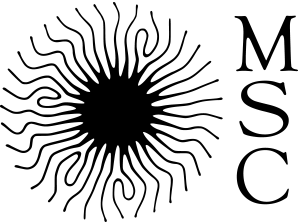
\includegraphics[scale=4]{figures/msc.png}\hspace{2cm}
%     
\includegraphics[scale=.13]{figures/anr-logo.png}\hfill
% }
%%%%%%%%%%%%%%%%%%%%%%%%%%%%%%%%%%%%%%%%%%%%%%%%%%%%%%%%%%%%%%%%%%%%%%%%%%%%%%%%

%%%%%%%%%%%%%%%%%%%%%%%%%%%%%%%%%%%%%%%%%%%%%%%%%%%%%%%%%%%%%%%%%%%%%%%%%%%%%%%%
%% Title page

% \makeatletter
% \setbeamertemplate{title page}{
%   \begin{minipage}[t][\paperheight]{\textwidth}
%     \ifx\inserttitle\@empty\else\usebeamertemplate*{title}\fi
%     \ifx\insertsubtitle\@empty\else\usebeamertemplate*{subtitle}\fi
%     \usebeamertemplate*{title separator}
%     \begin{center}
%     \ifx\beamer@shortauthor\@empty\else\usebeamertemplate*{author}\fi
%     \ifx\insertinstitute\@empty\else\usebeamertemplate*{institute}\fi
%     \ifx\insertdate\@empty\else\usebeamertemplate*{date}\fi
    
%     \end{center}
%     \vspace{.3cm}
%     \ifx\inserttitlegraphic\@empty\else\inserttitlegraphic\fi
%     %\vspace*{.2cm}
%   \end{minipage}
% }

%% FOOTLINE
\setbeamertemplate{footline}{
\leavevmode%

\hbox{\hspace*{-0.06cm}
\begin{beamercolorbox}[wd=.2\paperwidth,ht=2.25ex,dp=1ex,center]{author in head/foot}%
%\usebeamerfont{author in head/foot}\insertshortauthor\hfill
\insertframenumber{} / \inserttotalframenumber\hspace*{2ex}
\end{beamercolorbox}%

\begin{beamercolorbox}[wd=.6\paperwidth,ht=2.25ex,dp=1ex,center]{section in head/foot}%
\usebeamerfont{section in head/foot}%\insertshorttitle
\end{beamercolorbox}%

\begin{beamercolorbox}[wd=.2\paperwidth,ht=2.25ex,dp=1ex,right]{section in head/foot}%
%\usebeamerfont{section in head/foot}\hspace*{2em}
\usebeamerfont{section in head/foot}
%\insertframenumber{} / \inserttotalframenumber\hspace*{2ex}
\end{beamercolorbox}}%

\vskip0pt%
}
\makeatother

%%%%%%%%%%%%%%%%%%%%%%%%%%%%%%%%%%%%%%%%%%%%%%%%%%%%%%%%%%%%%%%%%%%%%%%%%%%%%%%%


